\documentclass[a4paper]{article}
\usepackage[utf8]{inputenc}
\usepackage[T2A]{fontenc}
\usepackage[12pt]{extsizes}
\everymath{\displaystyle}

\usepackage[english,russian]{babel}
\usepackage[left=10mm, top=10mm, right=10mm, bottom=20mm, nohead, nofoot]{geometry}
\usepackage{amsmath,amsfonts,amssymb} % математический пакет
\headsep=10mm

\usepackage{alltt}
\usepackage[most]{tcolorbox} % для управления цветом
% НАСТРОЙКИ
%теорема
\definecolor{theorem-color}{gray}{0.90} % уровень прозрачности (1 - максимум)
\newtcolorbox{htheorem}{colback=theorem-color,grow to right by=-4mm,grow to left by=-4mm,
    boxrule=0pt,boxsep=0pt,breakable} % настройки области с изменённым фоном

%определение
\definecolor{def-color}{gray}{0.98}
\newtcolorbox{definit}{colback=def-color,grow to right by=-4mm,grow to left by=-4mm,
    boxrule=0pt,boxsep=0pt,breakable} % настройки области с изменённым фоном

%доказательсвто теоремы
\definecolor{proof-color}{gray}{0.95} % уровень прозрачности (1 - максимум)
\newtcolorbox{hproof}{colback=proof-color,grow to right by=-1mm,grow to left by=-1mm,
    boxrule=0pt,boxsep=0pt,breakable} % настройки области с изменённым фоном

%замечания, следствия
\definecolor{consectary-color}{gray}{0.95} % уровень прозрачности (1 - максимум)
\newtcolorbox{cns}{colback=consectary-color,grow to right by=-4mm,grow to left by=-4mm,
    boxrule=0pt,boxsep=0pt,breakable} % настройки области с изменённым фоном



\usepackage{fancybox,fancyhdr}
\pagestyle{fancy}

\usepackage{hyperref}
\hypersetup{colorlinks=true, allcolors=[RGB]{010 090 200}} % цвет ссылок 
\newcommand{\lr}[1]{\left({#1}\right)} % команда для скобок

\author{Васильев Павел}
%\linespread{1}
\usepackage{amsmath}

\usepackage{graphicx}
\usepackage{ifpdf}
\ifpdf
\DeclareGraphicsRule{*}{mps}{*}{}
\fi
\usepackage{graphicx}
\usepackage{color}
\graphicspath{ {images/} }


\renewcommand{\headrulewidth}{0pt}

%\renewcommand{\familydefault}{\sfdefault}

\begin{document}

%\section*{HOW TO заботать собеседование в Яндекс на ML-стажировку}

\section*{Вопросы к собеседованию}

\subsection*{Линейные модели}

\begin{itemize}

\item \textit{Опишите задачу машинного обучния. Дайте определение объекту, целевой переменной, признакам, модели, функционалу ошибку}.

Объект - то, для чего мы хотим сделать какое-то предсказание. Целевая переменная - величина, которую мы хотим определять. Признаки - это набор характеристик для выборки объектов. Модель машинного обучения - это метод обучения компьютера, который позволяет выявить какие-то закономерности, благодаря которым сможет строить прогнозы целевой переменной. Функционал ошибки - функция, которая принимает на вход ответы алгоритма и правильные ответы и возвращает число, которое характеризует качество обученности модели.

\item \textit{Чем отличается функция потерь от функционала ошибки?}

Ничем.

\item \textit{Какие функции потерь используются при решении задачи регрессии?}

\begin{itemize}
\item \[ MSE(a, X) = \frac{1}{l} \sum_{i=1}^l (a(x_i) - y_i)^2 \]

MSE не сохраняет единицы измерения, например, если предсказывали цену в рублях, то MSE будет показывать рубли в квадрате.

\item \[ RMSE(a, X) = \sqrt{ \frac{1}{l} \sum_{i=1}^l (a(x_i) - y_i)^2 }\]

RMSE подходит для контроля качества во время обучения или для сравнения двух моделей, но не показывает то, насколько хорошо молель решает задачу. Типа если MSE = 100 и правильный ответ маленький по модулю, то эта ошибка слишком большая, а если правильный ответ > 100000, то такая ошибка очень маленькая.

\item Коэффициент детерминации $R^2$:

\[ R^2(a, X) = 1 - \frac{\sum_{i=1}^l (a(x_i) - y_i)^2}{\sum_{i=1}^l (y_i - \overline{y_i})^2}, \overline{y} = \frac{1}{l} \sum_{i=1}^l y_i \]

В числителе стоит дисперсия модели относительно правильных ответов, а в знаменателе общая дисперсия ответов.

Короче, это нормированная среднеквадратическая ошибка. Если эта ошибка близка к единице, это значит, что относительная дисперсия маленькая, значит модель хорошо описывает данные. А если близка к нулю, то модель похожа на константное предсказание.

\item \[ MAE(a, X) = \frac{1}{l} \sum_{i=1}^l |a(x_i) - y_i | \]

Модуль менее чувствителен к выбросам, но недифференцируем.
Но проблема недифференцируемости не сильно плохая (мы можем дополнить производную в точках разрыва какими-нибудь значениями). Основная проблема в том, что при градиентном спуске нам по функции потерь хочется понимать, насколько текущий прогноз модели близок к правильному ответу.

А производная модуля это функция $sign$, ну понятно.

\item HuberLoss:

\[ L_\delta(y, a) = \begin{cases}
\frac{1}{2} (y-a)^2, |y-a| < \delta \\
\delta \left( |y-a| - \frac{1}{2} \delta \right), |y-a| \geq \delta
\end{cases} \]

$\delta$ отвечает за то, что мы считаем за выбросы, а что нет.

\item Log-cosh:

\[ L(y, a) = \log \cosh (a-y) \]

Для маленьких отклонений здесь квадратичное поведение, для больших - линейное.

\item MSLE:

\[ L(y, a) = (log(a+1) - log(y+1))^2 \]

Подходит для задач с неотрицательным таргетом и неотрицательными прогнозами модели. Поскольку мы берём квадрат разностии именно логарифмов, то штрафуем мы за отклонения в порядке величин, а не в их значениях. И кстати, за заниженные прогнозы эта ошибка штрафует сильнее чем за завышенные, потому что логарифм.

\item MAPE, SMAPE

\[ L(y, a) = \left| \frac{y-a}{y} \right| \]

Эта функция ошибки заставляет нас не думать о масштабе данных, потому что мы нормируем по таргету отклонение. Но: если $y=1$ и все прогнозы $\geq 0$, то максимальная ошибка заниженного прогноза $=1$, а завышенного неограничена сверху.

Эту проблему решает SMAPE:

\[ L(y, a) = \frac{|y-a|}{\frac{|y|+|a|}{2}} \]
\end{itemize}

\item \textit{Запишите формулу для линейной модели регрессии}

\[ a(x) = w_0 + w_1 x + ... + w_d x_d \]

\[ a(x) = w_0 + \langle w, x \rangle \]

Ну часто $w_0$ включают в вектор $w$: $w = (w_0, ..., w_d)$, $a(x) = \langle w, x \rangle$ ($d$ - число признаков, $x = (1, x_1, ..., x_d)$ - признаковое описание объекта $x$.

\item \textit{Чем отличаются функционалы MSE и MAE? В каких случаях лучше использовать MSE, а в каких MAE?}

\[ MSE(a, X) = \frac{1}{l} \sum_{i=1}^l (a(x_i) - y_i)^2 \]
\[ MAE(a, X) = \frac{1}{l} \sum_{i=1}^l |a(x_i) - y_i | \]

MSE чувствителен к выбросам в данных, поскольку отклонение вносит вклад квадратично, MAE же просто смотрит на отклонение предсказание от ответа, поэтому он более терпим к выбросам, то есть обучая модель с MAE функцией ошибки, то мы  допускаем выбросы в датасете.

\item \textit{Чем отличается MAE от MAPE? Что более понятно заказчику продукта?}

\[ MAE(a, X) = \frac{1}{l} \sum_{i=1}^l |a(x_i) - y_i | \]
\[ MAPE(a, X) = \left| \frac{y-a}{y} \right| \]

MAPE позволяет работать с данными разного масштаба. При этом MAPE обладает особенностью: допустим у нас $y = 1$ и все прогнозы $\geq 0$, то максимальная ошибка заниженного прогноза равна 1, а завышенного не ограничена сверху.

\item \textit{Что такое коэффициент детерминации? Как интерпретировать его значения?}

\[ R^2(a, X) = 1 - \frac{\sum_{i=1}^l (a(x_i) - y_i)^2}{\sum_{i=1}^l (y_i - \overline{y_i})^2}, \overline{y} = \frac{1}{l} \sum_{i=1}^l y_i \]

Измеряет долю дисперсии, объяснённую моделью, в общей дисперсии таргета. Короче, это нормированная среднеквадратичная ошибка. Если дисперсия нашей модели такая же как и дисперсия таргета, то модель фиговая, а если дисперсия модели относительно дисперсии таргета мала, то модель неплохо предсказывает целевую переменную.

\item \textit{$log-cosh$ лучше функции потерь Хубера? Опишите обе функции потерь.}

Huber-loss:

\[ L_\delta(y, a) = \begin{cases}
\frac{1}{2} (y-a)^2, |y-a| < \delta \\
\delta \left( |y-a| - \frac{1}{2} \delta \right), |y-a| \geq \delta
\end{cases} \]

Log-cosh:

\[ L(y, a) = \log \cosh (a-y) \]

Log-cosh лучше Хубера тем, что у Хубера вторая производная разрывна. В остальном, они обе при маленьких отклонениях ведут себя квадратично, а при больших - линейно.

\item Что такое градиент? Какое его свойство используется при минимизации функций?

Градиент - вектор частных производных. Главное свойство - показывает направление наискорейшего возрастания функции. Находя градиент функции потерь по весам модели и двигаясь в противоположную сторону, мы уменьшаем ошибку.

\item \textit{Что такое градиентный спуск? Опишите процесс алгоритма.}

Градиентный спуск - итерационный алгоритм, который вот в чём заключается:

\begin{itemize}

\item Инициализируем $w^{(0)}$ как-нибудь

\item $w^{(k)} = w^{(k-1)} - \eta_k \nabla Q(w^{(k-1)})$, $\eta_k = \frac{1}{k}$

\end{itemize}

\item  Почему не всегда можно использовать полный градиентный спуск? Какие способы
оценивания градиента вы знаете? Почему в стохастическом градиентном спуске важно
менять длину шага по мере итераций? Какие стратегии изменения шага вы знаете?

Градиентный спуск не всегда можно использовать банально потому, что функция ошибки может быть недиферренцируемой.
Ещё это может быть связано с тем, что в некоторых местах функция ошибки близка к константе, и если в процессе градиентного спуска прийти в эту область, то он будет очень долго сходиться. Также градиентный спуск может не сойтись, если у нас сложная поверхность функции ошибки - несколько локальных минимумов.

Вот еще условия сходимости градиентного спуска: функция выпуклая и дифференцируемая, первая производная является липшицевой.

Полный град. спуск лучше не использовать, если объектов очень и очень много - он просто считаться долго будет.

Оценивание градиента:
как правило, функция ошибки представима в виде суммы ошибок на всех объектах:

\[ Q(w) = \frac{1}{l} \sum_{i=1}^l q_i(w) \]

Но можно не брать всю сумму, так как при большой выборке это слишком трудоёмкая операция, а можно оценивать весь градиент градиентом одного случайного объекта:

$\nabla_w Q(w) \approx \nabla_w q_{i_k} (w)$

$w^{(k)} = w^{(k-1)} - \eta_k \nabla q_{i_k} ( w^{(k-1)} ) $

Так как мы весь градиент оцениваем градиентом на одном объекте, то он может не замедляться вблизи точки минимума, так как параметры, оптимальные для всех объектов, могут не совпадать с параметрами для выбранного объекта. Поэтому необходимо самим уменьшать шаг стохастического градиентного спуска.

Шаг $\eta_k$ можно выбирать разным, главное, чтобы он удовлетворял условиям Роббинса-Монро:

\[ \sum_{k=1}^\infty \eta_k = \infty, \sum_{k=1}^\infty \eta_k^2 < \infty \]

Можно брать $\eta_k = \frac{1}{k}$, а можно $\eta_k = \lambda \left( \frac{s_0}{s_0+k} \right) ^k$, где $\lambda, s_0, p$ - параметры, $s_0 = 1, p = 0.5, d = 1$, $\lambda$ настраивается.

\item Что такое метод среднего стохастического градиента? В чём его плюсы относительно полного и стохастического градиентного спуска?

Метод заключается в следующем:

\begin{itemize}

\item Инициализируем как-нибудь $w^{(0)}$
\item Берём вспомогательную переменную $z_i^{(0)} = \nabla q_i (w^{(0)}), i = 1, ..., l$
\item На $k$-ой итерации берём случайный индекс $i_k$ и выполняем $z_i^{(k)} = \begin{cases}
\nabla q_i (w^{(k-1)}), if i = i_k \\
z_i^{(k-1)} else
\end{cases} $

\end{itemize}

И тогда $\nabla_w Q(w) \approx \frac{1}{l} \sum_{i=1}^l x_i^{(k)}$.

В этом методе мы обязаны хранить последние вычисленные градиенты для всех объектов выборки.

$w^{(k)} = w^{(k-1)} - \eta_k \sum_{i=1}^l z_i^{(k)}$


\item Какие модификации градиентного спуска еще есть?

\begin{itemize}

\item \textbf{Метод инерции (momentum).}

Если в обычном градиентном спуске у нас градиент сильно меняет направление от шага к шагу, то стоит его усреднить последними шагами. Для этого вводится 
\[ h_0 = 0 \]

\[ h_k = \alpha h_{k-1} + \eta_k \nabla_w Q(w^{(k-1)})\]

$\alpha$ отвечает за вклад градиентов с предыдущих шагов.

\item \textbf{AdaGrad, RMSprop.}

В методе AdaGrad предлагают сделать свою длину шага для каждой компоненты вектора параметров:

\[ G_{kj} = G_{k-1, j} + \left( \nabla_w Q(w^{(k-1)} ) \right)_j^2 \]

\[ w_j^{(k)} = w_j^{(k-1)} - \frac{\eta_t}{\sqrt{G_{kj}+\varepsilon}} \left( \nabla_w Q(w^{(k-1)}) \right)_j \]

\[ G_{k} = G_{k-1} + \left( \nabla_w Q(w^{(k-1)} ) \right)^2 \]

\[ w^{(k)} = w^{(k-1)} - \frac{\eta_t}{\sqrt{G_{k}+\varepsilon}} \left( \nabla_w Q(w^{(k-1)}) \right) \]


$\varepsilon$ нужен, чтобы корешок в ноль не превратился

Идея следующая: если мы вышли на плато по какой-то координате и соответствующая компонента градиента начала затухать, то нам нельзя уменьшать размер шага слишком сильно, так как мы рискуем на этом плато остаться, но в то же время уменьшать надо, потому что это плато может содержать оптимум. Если же градиент долгое время большой, то это может быть знаком, что нам нужно уменьшить размер шага, чтобы не пропустить оптимум. Поэтому мы стараемся компенсировать слишком большие или слишком маленькие координаты градиента.

Заметим, что $G_{kj}$ растёт, поэтому, шаги становятся всё медленнее, и градиентный спуск может остановиться раньше, чем нужно.

RMSprop использует экспоненциальное затухание градиентов:

\[ G_{kj} = \alpha G_{k-1,j} + (1-\alpha) \left( \nabla_w Q( w^{(k-1)}) \right)_j^2 \]

Тут уже размер шага по координате зависит от того, насколько быстро мы двигались по ней на последних шагах.

\item \textbf{Adam} 

Этот метод совмещает Momentum и AdaGrad (RMSprop):

\[ h_k = \beta_1 h_{k-1} + (1-\beta_1) \nabla_w Q( w^{(k-1)} )\]

\[ G_{k+1} = \beta_2 G_k + (1-\beta_2) \left( \nabla_w Q(w^{(k-1)}) \right)^2 \]

\[ w^{(k)} = w^{(k-1)} - \frac{\alpha}{\sqrt{(G_{k+1} + \varepsilon)}} h_{k-1}\]

\item \textbf{AdamW}

Добавим к Adam $l_2$ регуляризацию

\end{itemize}


\item \textit{Что такое переобучение? Как можно отследить переобучение модели?}

Переобучение - это состояние модели, когда на тренировочной выборке она показывает очень высокое качество, а на тестовой непозволительно низкое.

Как правило, когда модель переобученаа, мы можем посмотреть на её веса, и они оказываются большими по модулю. Фактически, это значит, что модель излишне подстроилась под обучющую выборку. Например, если у нас было несколько выбросов, то в линейной модели будут большие коэффициенты.

Также можно заметить переобучение с помощью валидационной выборки и кросс-валидации.

\item \textit{Что такое кросс-валидация? На что влияет количество блоков в кросс-валидации?}

Кросс-валидация - метод оценивания качества модели, который заключается в следующем: выборка делится на $k$ фолдов. Для каждого $1\leq i \leq k$ модель обучается на всех фолдах, кроме $i$-ого, а тестируется на $i$-ом. И берётся среднее со всех полученных ошикок. Таким образом, мы как будто увеличиваем размер выборки, и тестируем модель на немного разных входных данных. Вообще, кросс-валидация - частный случай бэггинга.

\item \textbf{Как построить итоговую модель после того, как по кросс-валидации подобраны
оптимальные гиперпараметры?}

\item \textit{Что такое регуляризация? Для чего используется?}

Регуляризация - способ борьбы с переобучением модели. Переобучение часто приводит к большим коэффициентам. Чтобы этого избежать, добавим ещё штраф за норму вектор весов:

\[ Q_\alpha (w) = Q(w) + \alpha R(w)\]

\[ R(w) = |w|_2 = \sum_{i=1}^d w_i^2 \]

\[ R(w) = |w|_1 = \sum_{i=1}^d |w_i| \]

Тут надо отметить, что $w_0$ регуляризовывать не надо, так как этот вес не связан с признаками объектов, он отвечает лишь за смещение модели.

\item \textit{Опишите, как работают L1- и L2-регуляризаторы.}

$L_1$ регуляризатор зануляет незначимые признаки. Это происходит потому, что если на плоскости с осями двух каких-то весов модели изобразить $|w|_1$, то она будет лежать внутри квадрата. Фукнция ошибки имеет эллипсовидные линии уровня, и вероятность того, что линия уровня (которая соответствует достаточно низкому значению функции ошибки) пройдёт через "угол" квадрата повыше, чем если линия уровня пересечёт квадрат где-то по-середине. А в углу квадрата одна из компонент вектора $w$ занулена. У $L_2$ регуляризации такого прикола нет, потому что норма ограничена окружностью, и там таких углов, как у квадрата, нет.
Ещё при $L_2$ регуляризации меньше шансов, что маленькие веса будут окончательно обнулены.

\item \textbf{Где используется метод максимального праводоподобия?}

\item \textit{Расскажите про метрики, которые штрафуют за перепрогноз сильнее, чем за
недопрогноз и наоборот(pinball loss)
}

MSLE:
\[ L(y, a) = (log(a+1) - log(y+1))^2 \]

Подходит для задач с неотрицательным таргетом и неотрицательными прогнозами модели. Поскольку мы берём квадрат разностии именно логарифмов, то штрафуем мы за отклонения в порядке величин, а не в их значениях. И кстати, за заниженные прогнозы эта ошибка штрафует сильнее чем за завышенные, потому что логарифм.

\item \textit{Расскажите про виды скейлинга. Зачем они нужны?}

Если не масштабировать данные, то в антиградиенте некоторые компоненты могут быть огромные, из-за чего спуск будет ковылять вокруг минимума, но не попадёт в него, потому что будет всё время перескакивать его. Можно даже уйти от минимума при неправильном подборе длины шага.

Масштабировать можно так:

\[ x_{ij} := \frac{x_{ij} - \mu_j}{\sigma_j}, \mu_j = \mathbb{E} x_{ij}, \sigma_j = \mathbb{D} x_{ij} \]

или так 

\[ x_{ij} := \frac{x_{ij} - \min_i x_{ij}}{max_i x_{ij} - min_i x_{ij}} \]

\item \textit{Как записываются аналитическое решения? Какие у них проблемы?}

\begin{equation}
\begin{gathered}
Loss = \frac{1}{n} (Xw -y)^T (Xw - y) = \\
= \{ a = Xw - y \} = \frac{1}{n} a^T a \\
\frac{\partial Loss}{\partial w} = \left( \frac{\partial a^T}{\partial w} a + a^T \frac{\partial a}{\partial w} \right) \frac{1}{n} = \\
= \frac{1}{n} \left( a^T \left( \left( \frac{\partial a}{\partial w} \right)^T \right)^T + a^T \frac{\partial a}{\partial w} \right) =  \\
= \frac{2}{n} \left( a^T \frac{\partial a}{\partial w} \right) = \frac{2}{n} a^T X = \frac{2}{n} \left( Xw-y \right)^T X = \frac{2}{n} \left( w^TX^TX-y^TX \right) = 0\\
w^T = y^TX (XTX)^{-1} \\
w = \left( y^TX (X^TX)^{-1} \right)^T\\
w = (X^TX)^{-1}X^Ty
\end{gathered}
\end{equation}

Проблемы: обращение матрицы - неустойчивая операция,

\end{itemize}


\subsection*{Классификация}

\begin{itemize}

\item \textit{Запишите формулу для линейной модели классификации. Что такое отступ?}

$\mathbb{Y} = \{ -1, 1 \}$

\[ a(x) = sgn \langle w, x \rangle \]

Ой, а если $\langle w, x \rangle = 0$?

Можем поступить так:
\begin{itemize}
\item Сказать, что такого никогда не бывает
\item Отказаться от классификации
\end{itemize}

Отступ:

\[ M_i = y_i \langle w, x_i \rangle \]

Знак отступка отражает корректность ответа классификатора, а его абсолютное значение - уверенность модели в своём ответе.

\item \textit{Как обучаются линейные классификаторы и для чего нужны верхние оценки пороговой функции потерь?}

Очевидным функционалом качества служит доля правильных ответов, тогда функция ошибки такая:

\[  Q(a, X) = \frac{1}{l} \sum_{i=1}^l [a(x_i) \neq y_i] \rightarrow \min_w \]

\[ Q(a, X) = \frac{1}{l} \sum_{i=1}^l [y_i \langle w, x \rangle < 0] \rightarrow \min_w \]

Эта функция некрасивая - она разрывная, градиентным спуском по ней не походишь - она всюду константа, кроме как в нуле. Поэтому придумали верхние оценки:

\begin{itemize}
\item $ \widetilde{L}(M) = \log (1+e^{-M}) $ - логистическая
\item $ \widetilde{L}(M) = \max(0, 1-M)$
\item $ \widetilde{L}(M) = e^{-M}$ - экспоненциальная
\item $ \widetilde{L}(M) = \frac{2}{1+e^M}$ - сигмоидная
\end{itemize}

\item \textit{Что такое точность, полнота и F-мера? Почему F-мера лучше арифметического среднего и минимума?}

Точность (precision) - показывает, какая доля объектов, выделенных классификатором как положительные, реально положительные.

Полнота (recall) - показывает, какая часть положительных объектов была выделена классификатором.

\[ precision = \frac{TP}{TP+FP} \]

\[ recall = \frac{TP}{TP+FN} \]

Это две метрики, хотим оптимизировать одну.

Допустим берём среднее арифметическое. Тогда модель с ужасным precision и большим recall покажет такую же метрику как модель с средненьким precision и recall. Так не пойдёт.

Допустим берём минимум. Тогда считается, что если recall больше чем precision, то модели с равным recall и любым precision будут считаться одинаковыми по качеству, но это совсем не так.

F-мера - это сглаженная версия минимума:

\[ F = \frac{2 \cdot precision \cdot recall}{precision + recall} \]

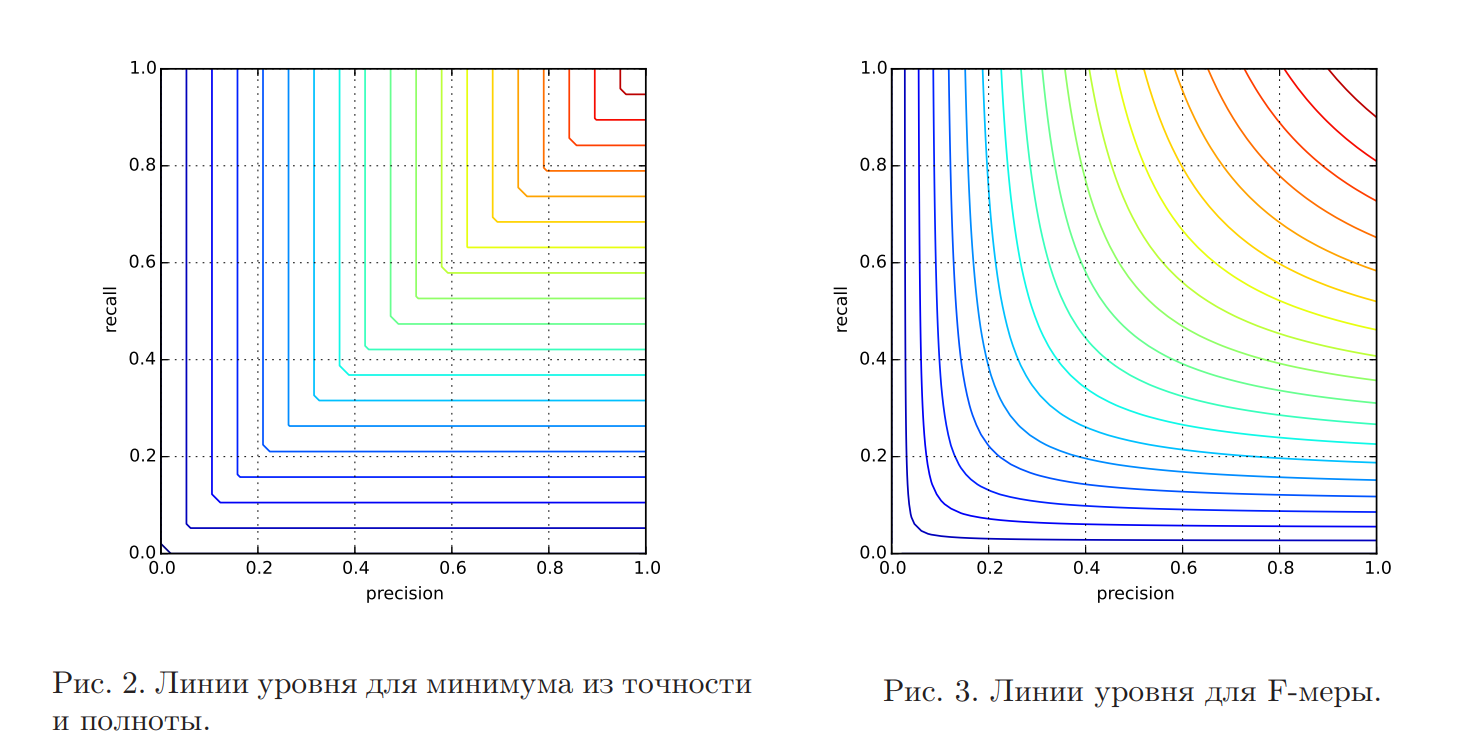
\includegraphics[width=18cm]{f-measure.png}

Кстати, есть ещё R-точность. Она равна точности при таком пороге $t$, при котором полнота равна точности:

\[ t* = argmin_t |precision(sign(b(x)-t)) - recall(sign(b(x) - t))| \]

\[R-precision = precision(sign(b(x)-t*))\]

То есть R-precision равна точности при таком пороге, при котором количество отнесённых к положительному классу объектор равно фактическому количеству положительных объектов в выборке.

Ещё есть lift. Есть задачи, связанные с выбором подмножества: выделение лояльных клиентов банка, обнаружение уходящих пользователей мобильного оператора и т.д. Заказчика может интересовать вопрос, насколько выгоднее работать с этим подмножеством по сравнению со всем множеством.
Интерпретируется lift как улучшение доли положительных объектов в подмножестве относительно доли в случайно выбранном подмножестве такого же размера.

\[ lift = \frac{precision}{\frac{TP+FN}{l}} \]

\item \textit{Для чего нужен порог в линейном классификаторе? Из каких соображений он может
выбираться?}

Порог нужен, чтобы определять баланс между precision и recall в зависимости от того, чего мы хотим добиться.
Может мы хотим минимизировать ложноположительные результаты или наоборот ложноотрицательные.

\item \textit{Что такое AUC-ROC? Опишите алгоритм построения ROC-кривой.}

AUC-ROC - метрика, не зависящая от порога, в отличие от выше описанных.
\[ FPR = \frac{FP}{FP+TN} \]

\[ TPR = \frac{TP}{TP+FN} \]

Отсортируем объекты по $\langle w, x \rangle$ и будем перебирать порог $t$ в $a(x) = sign(\langle w, x \rangle - t)$ и отмечать точки $(FPR, TPR) = (FPR, precision)$.

ROC-AUC равна площади под получившимся графиком
AUC-ROC интерпретируется как вероятность того, что для случайно выбранных положительного объекта $x_+$ и отрицетельного $x_-$ будет выполнено $b(x_+) > b(x_-)$.


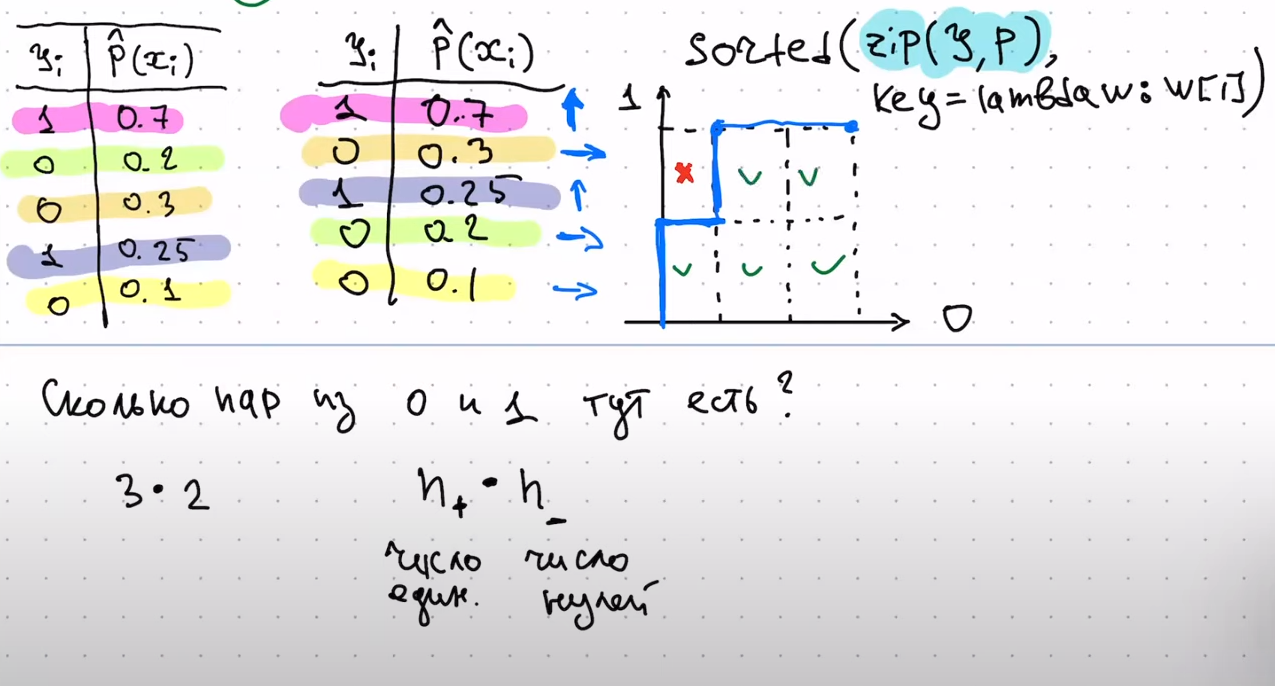
\includegraphics[width=18cm]{auc-roc.png}

Что делать, если:
$y = 1, p  = 0.5$

$y = 0, p = 0.5$

Тогда делаем один шажок по диагонали вверх-направо. 

Кстати AUC-ROC тоже чувствителен к дисбалансу классов.

Что будет с ROC-AUC, если умножить все скоры:

\begin{itemize}
\item на 2

Ответ: ничего не изменится, так как на порядок не повлияет
\item на 0.5

Ответ: аналогично
\item на -1

Ответ: порядок поменяется на противоположный. А площадь станет равной 1 - ROC-AUC.

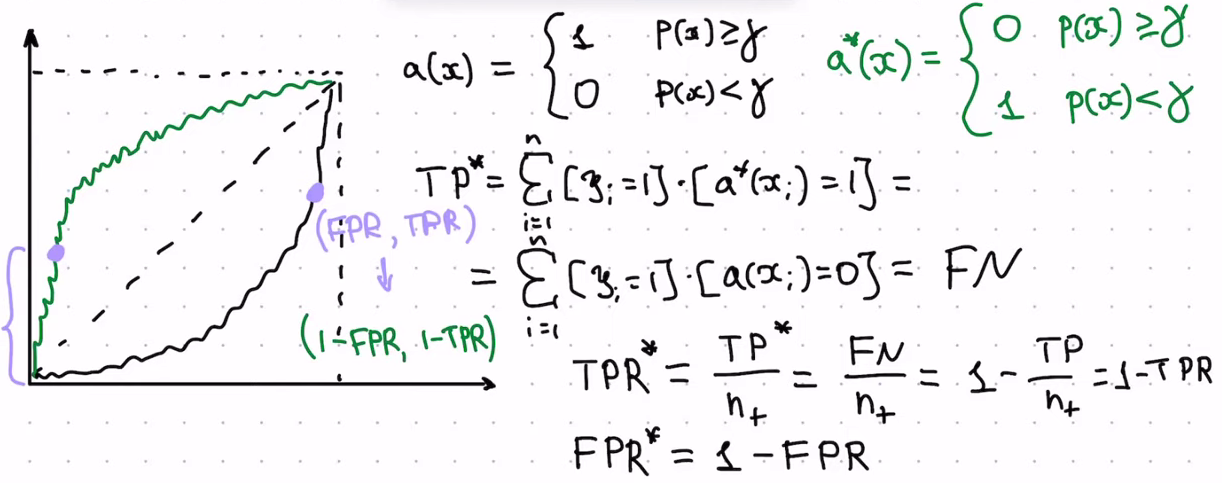
\includegraphics[width=15cm]{auc-roc-q.png}
\end{itemize}

Упражнение:

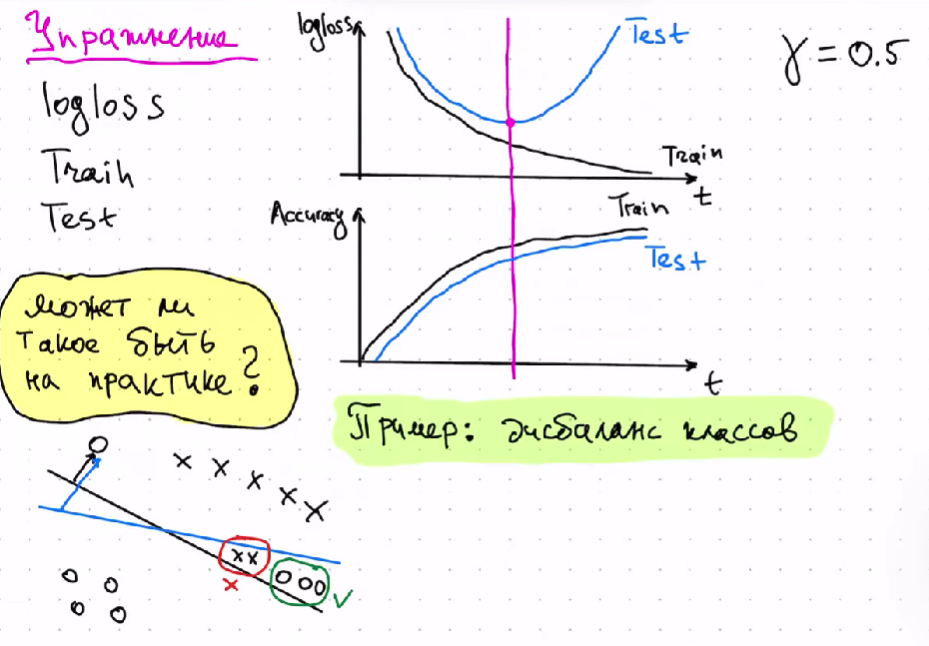
\includegraphics[width=15cm]{logloss-q.png}

Что будет, если с ROC-AUC удалить 10 процентов объектов первого класса?

Изменится, но непонятно как. Изменится, так как общее количество пар уменьшится. Если убрались плохие пары, то ROC-AUC улучшится, если убрались только хорошие пары, то ROC-AUC уменьшится. Иначе непонятно.

\item \textit{Что такое AUC-PRC? Опишите алгоритм построения PR-кривой.}

Идея та же, что и в AUC-ROC, только откладываем $(recall, precision)$. Только тут уже нет проблемы с несбалансированными классами.

\item \textit{. Что означает “модель оценивает вероятность положительного класса”? Как можно
внедрить это требование в процедуру обучения модели?}

Если говорят, что модель уверена в ответе на $95$ процентов, то если взять все объекты с $95$ процентов, то $95$ процентов из них будут положительными.

Классификатор $b$ верно оценивает вероятности, если при $P$ мы возьмём все $x \in \mathbb{X}$ с $b(x) = P$ и среди них доля положительных равна $P$.

Мы допускаем, что для одинакового признакового описания ответ будет разный. Причём если устремлять количество таких объектов в бесконечность, то доля положительных будет стремиться к $p(y=+1|x)$.

То есть хотим $argmin_{b \in \mathbb{R}} \frac{1}{n} \sum_{i=1}^n L(y_i, b) \approx p(y=+1|x)$

А если устремить $n \rightarrow +\infty$, то 
\[ argmin_{b \in \mathbb{R}} \mathbb{E} L(y, b) \approx p(y=+1|x) \]

\item \textit{Запишите функционал логистической регрессии. Как он связан с методом максимума
правдоподобия?}

\[ Q(a, X) =  \sum_{i=1}^l \log (1+\exp(-y_i \langle w, x_i \rangle )\]

Если наш алгоритм $b$ выдает вероятности, то вероятность того, что в выборке встретится $x_i$ с классом $y_i$ равна $b(x)^{[y+i = +1]}\cdot (1-b(x_i))^{[y_i=-1]}$

\[ Q(a, X) = \prod_{i=1}^l b(x)^{[y_i = +1]}\cdot (1-b(x_i))^{[y_i=-1]} \]

Логарифмируем:

\[ - \sum_{i=1}^l \left( [y+i = +1] \log b(x_i) + [y_i = -1] \log (1-b(x_i) \right) \rightarrow \min \]

Давайте преобразуем ответы $b$, чтобы он отдавал ответы в $[0,1]$:

\[ p(y=1|x) - \frac{1}{1+\exp(-\langle w, x \rangle)} \]

\[ Q(a, X) = - \sum_{i=1}^l \left( [y_i = +1] \log \frac{1}{1+\exp(-\langle w, x_i \rangle)} + [y_i = -1] \log \frac{\exp(-\langle w, x_i \rangle)}{1 + \exp(-\langle w, x_i \rangle)} \right) = \]

\[
= - \sum_{i=1}^l \left( [y_i = +1] \log \frac{1}{1+\exp(-\langle w, x_i \rangle)} + [y_i = -1] \log \frac{1}{1 + \exp(\langle w, x_i \rangle)} \right) = 
\]

\[ = \sum_{i=1}^l \log \left( 1+\exp(-y_i \langle w, x_i \rangle) \right) \]

\item \textbf{Когда используется accuracy?}

\item \textbf{Как бороться с дисбалансом классов?}


\end{itemize}

\section*{Многоклассовая классификация}

\begin{itemize}

\item \textit{Как измеряется качество в задаче многоклассовой классификации?}

Как делали: в бинарной классификации строили линейную модель $b(x) = \langle w, x \rangle + w_0$, а потом накидывали $\sigma(z) = \frac{1}{1+\exp(-z)}$. Теперь мы построили $K$ линейных моделей $b_k(x) = \langle w_k, x \rangle w_{0k}$.

Для оценки вероятности тут стоит использовать $SoftMax$, которая производит нормировку вектора:

\[ SoftMax(z_1, ..., z_K) \left( \frac{\exp(z_1)}{\sum_{k=1}^K \exp(z_k)}, ...,  \frac{\exp(z_K)}{\sum_{k=1}^K \exp(z_k)} \right) \]

Тогда вероятность $k$-ого класса будет выражаться как 

\[ P(y=k|x, w) = \frac{\exp(\langle w_k, x \rangle + w_{0k})}{\sum_{j=1}^K \exp( \langle w_j, x \rangle + w_{0j} )} \]

Обучается такая модель с помощью метода максимального правдоподобия:

\[  \sum_{i=1}^l \log P(y=y_i | x_i, w) \rightarrow \max_{w_1, ..., w_K} \]

\item \textbf{Расскажите микро и макро-усреднение?}

\item \textit{Что такое mean-target encoding?  Может ли mean-target encoding может привести к переобучению? Как можно этого
избежать?}

Mean-target кодирование заключается в том, что для категориальных признаков мы можем прокидывать таргет прямо в признак: вместо категории вписать среднее значение таргета при этой категории. Очевидно, тут происходит переобучение, потому что по факту мы ответ помещаем в датасет, на котором обучаем модель. С этой проблемой помогает справиться регуляризация, как всегда.

\item \textit{Что такое решающее дерево?}

Это бинарное дерево, в котором:

\begin{itemize}
\item Каждой вершине $v$ приписан предикат $B_v: \mathbb{X} \rightarrow \{ 0, 1 \}$
\item Каждому листу $v$ приписан прогноз $c_v \in \mathbb{Y}$
\end{itemize}

Для каждого объекта из $\mathbb{X}$ стартуем из корня, считаем $B_v$ и если $B_v(x) = 1$ спускаемся в левого сына, иначе в правого. Идём, пока не достигнем лист, а затем считаем прогноз.

Обычно предикат простой:
\[ B_v(x, j, t) = [x_j \leq t] \]

\item \textit{ Опишите жадный алгоритм обучения решающего дерева.}

$X_m$ - множество объектов, которые попали в текущий лист. Тогда алгоритм такой:

\item Создаём вершину $v$
\item Если выполнен критерий остановки $Stop(X_m)$, то возвращаем $Ans(X_m)$
\item Иначе находим предикат $B_{j, t}$, который определит наиилучщее разбиение такого множество на две подвыборки $X_l$, $X_r$, максимизируя критерий ветвления $Branch(X_m, j, t)$
\item Запустимся от $X_l$ и $X_r$.


$Ans(X_m)$ - вычисляет ответ для листа по попавшим туда ответам: меткой самого частого класса (в классификации), средним, медианой или др. в линейной регрессии.

$Stop(X_m)$ - функция, которая решает, продолжить алгоритм или пора остановиться (глубина, число листов, однородность объектов в листе и др.).

$Branch(X_m, feature, value)$ - функция, оценивающая, насколько хорош сплит.

Есть такая штука, как impurity:

\[ H(X_m) = \min_{x \in \mathbb{Y}} \frac{1}{|X_m|} \sum_{(x_i, y_i) \in X_m} L(y_i, c) \]

Чем ниже эта функция, тем лучше объекты в листе можно приблизить константой. Давайте для пня введём информативность:

\[ \frac{1}{|X_m|} \left( \sum_{x_i \in X_l} L(y_i, c_l) + \sum_{x_i \in X_r} L(y_i, c_r) \right) \]

\[ \frac{1}{|X_m|} \left( \sum_{x_i \in X_l} L(y_i, c_l) + \sum_{x_i \in X_r} L(y_i, c_r) \right) = 
\frac{1}{|X_m|} \left( |X_l| \frac{1}{|X_l|} \sum_{x_i \in X_l} L(y_i, c_l) + |X_r| \frac{1}{|X_r|} \sum_{x_i \in X_r} L(y_i, c_r) \right) =\]
\[ =  \frac{|X_l|}{|X_m|} H(X_l) + \frac{|X_r|}{|X_m|}H(X_r)\]

Посмотрим на impurity в регрессии с MSE:

$L(y_i, c) = (y_i-c)^2$

\[ H(X_m) = \frac{1}{|X_m|} \min_{c \in \mathbb{Y}} \sum_{(x_i, y_i) \in X_m} (y_i - c)^2 \]

\[ c = \frac{\sum y_i}{|X_m|} = \overline{y} \]

\[ H(X_m) =  \min_{c \in \mathbb{Y}} \sum_{(x_i, y_i) \in X_m} \frac{(y_i - \overline{y})^2}{|X_m|} \]


Оценка для значения в каждом листе - среднее, а выбираем сплит, минимизируя дисперсию в листе.

С MAE лучшее константное предсказание даёт медиана:

\[ H(X_m) = \sum_{(x_i, y_i) \in X_m} \frac{|y_i - MEDIAN(Y)|}{|X_m|} \]

\textbf{Критерий информативности в задаче классификации: missclassification error}

Имеем $K$ классов, $p_k$ - доля объектов класса $k$ в вершине $X_m$:

\[ p_k = \frac{1}{|X_m|} \sum_{(x_i, y_i) \in X_m} \mathbb{I}[y_i = k] \]

Для простоты пусть $L(y_i, c) = \mathbb{I}[y_i \neq c] $

\[ H(X_m) = \min_{x \in Y} \frac{1}{|X_m|}  \sum_{(x_i, y_i) \in X_m} \mathbb{I} [y_i \neq c ] \]

Оптимальное предсказание $k*$ - это самый популярный класс:

\[ H(X_m) = \min_{x \in Y} \frac{1}{|X_m|}  \sum_{(x_i, y_i) \in X_m} \mathbb{I} [y_i \neq k* ] = 1 - p_{k*}\]

А сейчас хотим предсказывать распределение классов $(c_1, ..., c_K)$. Будем максимизировать логарифм правдоподобия:

\[ P(y|x, c) = P(y|c) = \prod_{(x_i, y_i) \in X_m} P(y_i|c) = \prod_{(x_i, y_i) \in X_m} \prod_{k=1}^K c_k^{\mathbb{I}[y_i=k]}\]

\[ H(X_m) = \min_{\sum_k c_k = 1} \left( -\frac{1}{|X_m|} \sum_{(x_i, y_i) \in X_m} \sum_{k=1}^K \mathbb{I} [y_i = k] \log c_k \right)\]

Чтобы минимизировать $H(X_m)$, надо брать $c_k = p_k$.

Почему?

Условие такое: $\sum c_k = 1$

Минимизируем Лагранжиан 

\[ \min_{c, \lambda} \left( \left( -\frac{1}{|X_m|} \sum_{(x_i, y_i) \in X_m} \sum_{k=1}^K \mathbb{I} [y_i = k] log c_k \right) + \lambda \sum_{k=1}^K c_k \right) \]

\[ 0 = \frac{\partial }{\partial c_j} L(c, \lambda) = \left( \left( -\frac{1}{|X_m|} \sum_{(x_i, y_i) \in X_m} \mathbb{I} [y_i = j] \frac{1}{c_j} \right) + \lambda  \right) = -\frac{p_j}{c_j} + \lambda \]

\[ c_j = \frac{p_j}{\lambda} \]

\[ 1 = \sum_{k=1}^K c_k = \frac{1}{\lambda} \sum_{k=1}^K p_k = \frac{1}{\lambda} \Rightarrow \lambda = 1 \Rightarrow c_k = p_k \]

Тогда информативность принимает вид 

\[ H(X_m) = - \sum_{k=1}^K p_k \log p_k \]
Это энтропия.

Есть ещё \textbf{критерий Джини}.

Можно вместо логарифма правдоподобия брать метрику Бриера (это MSE от вероятностей):

\[ H(X_m) = \min_{\sum_k c_k = 1} \frac{1}{|X_m|} \sum_{(x_i, y_i) \in X_m} \sum_{k=1}^K ( c_k - \mathbb{I}[y_i=k] )^2 \]

Оптимальное значение $H(X_m)$ достигается при $p_j = \frac{1}{|X_m|} \sum_i \mathbb{I} [y_i = j]$

Тогда $H$ примет вид 

\[ H(X_m) = \sum_{k=1}^K p_k (1-p_k) \]

\item \textit{Почему с помощью бинарного решающего дерева можно достичь нулевой ошибки на обучающей выборке без повторяющихся объектов?}

Потому что мы можем сделать так, чтобы в лист попадал один объект.

\item \textit{В чем отличия энтропийного критерия и критерия Джини?}

Это две метрики для выбора способа разбить дерево. Измерение индекса Джини - это вероятность того, что случайная выборка будет классифицирована неправильно, если мы случайным образом выберем класс в соответствии с распределением в ветке дерева.

Энтропия - это мера информации (точнее ее отсутствия). Вы рассчитываете прирост информации, делая разбиение. В этом энтропия отличается, это измерение того, как вы уменьшаете неопределенность относительно класса.


\item \textit{Как связаны линейные модели и решающие деревья?}

Дерево разбивает признаковое пространство на непересекающиеся множества $\{ J_1, ..., J_n \}$,  и в каждом множестве выдаёт свой константный прогноз $w_j$. Значит алгоритм записывается как 

\[ a(x) = \sum_{j=1}^n w_j [x \in J_j] \]

Это линейная модель над признаками $([x \in J_j])_{j=1}^n$. Решающее
дерево с помощью жадного алгоритма подбирает преобразование признаков для данной задачи, а затем просто строит линейную модель над этими признаками.

\item \textit{В чем заключается метод опорных векторов?}

Идея заключается в построении гиперплоскости, разделяющей объекты выборки оптимальным способом. Алгоритм работает в предположении, что чем больше расстояние (зазор) между разделяющей гиперплоскостью и объектами разделяемых классов, тем меньше будет средняя ошибка классификатора.

\item \textit{Нужно ли заниматься предобработкой данных в случае дерева?}

Деревья умеют работать с категориальными признаками. Пусть $C = \{x_1, ..., c_M\} $. Пытаясь разбить $C$ на $C_l$ и $C_r$ мы перебираем $2^{M-1}-1$ сплитов (долго). Утверждается, что для бинарной классификации $c_m$ можно упорядочитьь по неубыванию доли объектов класса 1 и работать с ними как с вещественными признаками.
Для регрессии с MSE $c_m$ можно упорядочивать по среднему значению таргета.


\item \textit{Как деревья работают с Nan?}

Идея в том, что 
классифицируемый объект относится к тому классу, которому принадлежат ближайшие к нему объекты обучающей выборки.

\item \textit{Как деревья работают с категориальными значениями?}

Пусть $V_m$ - это подмножество $X_m$, состоящее из пропущенных значений.

Можно так поступить:

\begin{itemize}
\item В момент выбора сплита игнорируем объекты из $V_m$, а когда уже нашли нужный сплит, отправим эти объекты в обеих сыновей с весами $\frac{|X_l|}{|X_m|}$ и $\frac{|X_r|}{|X_m|}$. В итоге с поддеревьев мы получим ответ $\hat{y_l}$ и $\hat{y_r}$ и возьмём $\hat{y} = \frac{|X_l|}{|X_m|} \hat{y_l} + \frac{|X_r|}{|X_m|} \hat{y_r}$

\item Можно их просто не учитывать никак
\end{itemize}

\item \textit{ Как сделать многоклассовую классификацию через логрег?}

Хотим предсказывать распределение классов $(c_1, ..., c_K)$. Будем максимизировать логарифм правдоподобия:

\[ P(y|x, c) = P(y|c) = \prod_{(x_i, y_i) \in X_m} P(y_i|c) = \prod_{(x_i, y_i) \in X_m} \prod_{k=1}^K c_k^{\mathbb{I}[y_i=k]}\]

\[ H(X_m) = \min_{\sum_k c_k = 1} \left( -\frac{1}{|X_m|} \sum_{(x_i, y_i) \in X_m} \sum_{k=1}^K \mathbb{I} [y_i = k] \log c_k \right)\]

Чтобы минимизировать $H(X_m)$, надо брать $c_k = p_k$.

Тогда информативность принимает вид 

\[ H(X_m) = - \sum_{k=1}^K p_k \log p_k \]

\item \textit{Приведите пример семейства алгоритмов с низким смещением и большим разбросом}

Линейные модели, градиентный бустинг.

\item \textit{Приведите пример семейства алгоритмов с большим смещением и низким разбросом.}

\item \textit{Что такое бэггинг? Как его смещение и разброс связаны со смещением и разбросом
базовых моделей?}

Представим, что есть $X = (x_i, y_i)_{i=1}^l$

Бутстрап: генерация подвыборки из $X$ выбором $l$ объектов с возврашением.

Из $X$ сгенерируем $X_1, ..., X_n$ подвыборок. И допустим мы обучили $b_1(x), ..., b_N(x)$ на своих подвыборках.

$y(x)$ - истинные объекты, $p(x)$ - плотность на $X$

Посчитаем ошибку $\varepsilon_j(x) = b_j(x) - y(x)$

\[ \mathbb{E} (b_j(x) - y(x))^2 = \mathbb{E} \varepsilon_j^2(x) \]

Предположим, что $\mathbb{E} \varepsilon_j^2(x) = 0$ и $\mathbb{E} \varepsilon_j(x)  \varepsilon_i(x) = 0, i \neq j$ - некореллированность ошибок.

Тогда создадим новую модель

\[ a(x) = \frac{1}{N} \sum_{j=1}^N b_j(x) \]

\begin{equation}
\begin{gathered}
\mathbb{E} (a(x)-y(x))^2 = \mathbb{E} \left( \frac{1}{N} \sum_{j=1}^N b_j(x) - \frac{1}{N} \sum_{j=1}^N y(x) \right)^2 = \mathbb{E} \left( \frac{1}{N} \sum_{j=1}^N \varepsilon_j(x) \right)^2 = \\
= \frac{1}{N^2} \mathbb{E}\left( \sum_{j=1}^N \varepsilon_j^2(x) + \sum_{i \neq j} \varepsilon_i(x) \varepsilon_j(x)  \right) = \frac{1}{N^2} \mathbb{E} \sum_{j=1}^N \varepsilon_j^2(x) = \frac{1}{N^2} N \mathbb{E}_1 = \frac{\mathbb{E}_1}{N}
\end{gathered}
\end{equation}

Чекайте, усреднение $N$ моделей уменьшает матожидание ошибки в $N$ раз.

$X = (x_i, y_i)_{i=1}^l, y_i \in \mathbb{R}$

$p(x, y)$ на $\mathbb{X} \times \mathbb{Y}$ - плотность.

$L(y, a) = (y-a)^2$

Среднеквадратичный риск: $R(a) = \mathbb{E}_{x, y} (y-a(x))^2 = \iint_{X \times Y} (y-a(x))^2 p(x, y) dxdy$

\[ a_*(x) = \mathbb{E} (y|x) = \int_\mathbb{Y} yp(y|x) dy \]

Метод обучения:

$\mu: (\mathbb{X} \times \mathbb{Y})^l \rightarrow \mathbb{A}$

$\mu$ переводит из пространства обучающих выборок в семейство моделей.

$\mu(X)$ - модель, $\mu(X)(x)$ - ответ модели.

\[ L(\mu) = \mathbb{E}_X \mathbb{E}_{x, y} (y - \mu(X)(x))^2 \]
Это ошибка метода обучения.

\begin{equation}
\begin{gathered}
L(\mu) = \mathbb{E}_{x, y} \left( \left( y - \mathbb{E}(y|x) \right)^2 \right) + \\
+ \mathbb{E}_x \left( \left(\mathbb{E}_X \mu(X) - \mathbb{E} (y|x) \right)^2 \right) + \\
+ \mathbb{E}_x \mathbb{E}_X \left( \mu(X) - \mathbb{E}_X \mu(X) \right)^2
\end{gathered}
\end{equation}

$\mathbb{E}(y|x)$ - лучшая модель,

$\mathbb{E}_{x, y} \left( \left( y - \mathbb{E}(y|x) \right)^2 \right)$ - ошибка лучшей модели (или шум).

$\mathbb{E}_x \left( \left(\mathbb{E}_X \mu(X) - \mathbb{E} (y|x) \right)^2 \right)$ - смещение. Тут мы берём лучшую модель и берём среднюю модель по всем обучающим выборкам. И смотрим, насколько они отклоняются. Показывает то, насколько впринципе можно угадать истинную закономерность. Если средняя модель не может собой приблизить лучшую модель, значит наща модель не лучшим образом выбрана.

$\mathbb{E}_x \mathbb{E}_X \left( \mu(X) - \mathbb{E}_X \mu(X) \right)^2$ - разброс. Берём конкретную модель, обученную на $X$, смотрим её отклонение от средней модели, а дальше эти отклонения усредняем по всем обучающим выборкам. По сути эта штука показывает то, насколько в среднем мои модели на разных обучающих выборках отклоняются от средней модели. В общем, если у нас прогнозы не сильно меняются, если модели пихать изменённые выборки, то она устойчива, и это хорошо.

\item \textit{Что такое случайный лес? Чем он отличается от бэггинга над решающими
деревьями?}

Случайный лес - несколько деревьев.

\begin{itemize}
\item Деревься обучаются с min sample leaf = 3
\item Деревья обучаются на бутстрапированных подвыборках
\item К важдой вершину в $[x_j = t]$ $j$ выбирается из случайного подмножества признаков размера $k$.
\end{itemize}

Для регрессии ответ модели 

\[ \frac{1}{N} \sum b_n(x) \]

Для классификации

\[ argmax_{y \in Y} \sum_{n=1}^N [b_n(x) = y] \]

\item \textit{Перечислите основные плюсы решающего леса}

Не переобучается.

\item \textit{Назовите недостатки случайного леса.}

\begin{itemize}
\item Очень долго обучается
\item Если смещение дерева сильно большое, то случайный лес будет плох
\end{itemize}

\item \textit{Как работает алгоритм градиентного бустинга}

Каждая следующая модель корректирует ошибки предыдущих

Пример: бустинг для регрессии:

\[ \frac{1}{l} \sum_{i=1}^l (a(x_i) - y_i)^2 \rightarrow \min_a \]

\[a_N(x) = \sum_{n=1}^N \gamma_n b_n(x), \gamma_n \in \mathbb{R} \]

Обучаем первое дерево:
\[ b_1(x): \frac{1}{l} \sum_{i=1}^l (b_1(x_i)-y_i)^2 \rightarrow \min_{b_1} \]

Желаем слудующее:

\[ b_2(x): \quad b_1(x_i) + b_2(x_i) = y_i \]
\[ b_2(x_i) = y_i - b_1(x_i) = s_i \]
\[ \frac{1}{l} \sum_{i=1}^l (b_2(x_i)-s_i)^2 \rightarrow \min_{b_2} \]

\[ \gamma_2 = argmin_{\gamma \in \mathbb{R}} \frac{1}{l} \sum_{i=1}^l \left( b_1(x_i) + \gamma b_2(x_i) - y_i \right)^2 \]


\item \textit{ Как обычно выглядят базовые модели в бустинге. Опишите почему?}

Обычно базовая модель достаточно слабая (дерево глубины 2). Это нужно для того, чтобы она не переобучилась сразу же. Потому что если она переобучится, следующие модели, которые призваны корректировать ошибку первой, будут в таком случае бесполезны.

\item \textit{Что такое сдвиги в градиентном бустинге, зачем они нужны?}

Сдвиг в градиентном бустинге - это $z$ в следующей функции ошибки:

\[ \frac{1}{l} \sum_{i=1}^l L(y_i, a_{N-1}(x_i)+ z) \]

Этот сдвиг нужен, чтобы определить, как надо подкорректировать $a_{N-1}$, чтобы ошибку уменьшить.

\item \textit{Как обучается очередной базовый алгоритм в градиентном бустинге?}

Пусть $s_i = - \frac{\partial}{\partial z} L(y_i, z) |_{z=a_{N-1}(x_i)}$

$\frac{1}{l} \sum_{i=1}^lv(B_N(x_i) - s_i)^2 \rightarrow \min_{b_N}$

$a_N(x) = a_{N-1} (x) + b_N(x)$


Почему мы в $\frac{1}{l} \sum_{i=1}^lv(B_N(x_i) - s_i)^2 \rightarrow \min_{b_N}$ берём не исходную функцию потерь, а квадрат?

Функция потерь уже как-то учтена в $s_i$, поскольку это значение производной исходной функции потерь в какой-то точке. Кроме того, функция потерь рассчитана на единицах изменения, в которых считается целевая переменная. Если изначальный таргет был в рублях, то производная от рублей уже точно не рубли. Будет странно, если функцию потерь про рубли мы будем применять к чему-то совершенно другому.

Хороший вопрос: почему нельзя просто взять $b_1(x)$ и прибавлять на каждом шаге $a_{N-1} (x_i) + s_i$? Зачем нам прям модель $b_N$ обучать после каждого шага? Потому что непонятно, как быть с новыми объектами. Если бы мы пустили градиентный спуск просто, то вообще непонятно, как получать прогноз на новых данных. А если после каждого шага град спуска обучать модель, то для нового объекта ответ будет как полученная композиция моделей.

\item \textit{Как работает oob?}

Oob нужен для оценивания качества случайного леса.

Идея:

$b_n(x)$ обучается на $X_n \subset X$.

\[ DOB = \frac{1}{l} \sum_{i=1}^l L(y_i, \frac{1}{\sum_{n=1}^N [x_i \not\in X]} \sum_{n=1}^N [x_i \in X] b_n(x) \]

$\frac{1}{\sum_{n=1}^N [x_i \not\in X]} \sum_{n=1}^N [x_i \in X] b_n(x)$ - это прогноз для $x_i$ по деревьям, которые на $x_i$ не обучались.

\item \textit{Как работает feature importance?}

Важности признаков (перестановочные).

$a(x)$ - модель (не обязательно случайный лес).

$Q(a, X_{test}) = Q_{test}$

Интересует важность $j$-ого признака.

Берём в $X_{test}$ $j$-ый столбец и перемешиваем все значения в нём - получится $X_{test}^{(j)}$

$Q(a, X_{test}^{(j)}) = Q_{test}^{(j)}$

Если мы перемешали столбец и качество модели от этого не поменялось, значит этот признак не сильно и был важен для предсказания таргета.

Важность $j$-ого признака: $Q_{test}^{(j)} - Q_{test} = q_i$

\begin{itemize}

\item $q_i \approx 0 \Rightarrow$ признак неважный

\item $q_i > 0 \Rightarrow$ прищнак важный

\item $q_i < 0 \Rightarrow $ WTF?
\end{itemize}

\item \textit{Расскажите про виды бустинга(catboost, lgbm, xgb), их особенности и различия}

\begin{itemize}

\item \textbf{Catboost}

Под капотом содержится:
\begin{itemize}

\item Симметричные забывчивые деревья.

\begin{enumerate}
\item Значительно ускорены по сравнению с послойным построением дерева.

\item Уменьшенное переобучение.

\item Устойчиво к изменению гиперпараметров.
\end{enumerate}
В каждом узле на одном и том же уровне дерева используется одна и та же точка расщепления.

\item Обработка категориальных признаков

Способы:
\begin{enumerate}

\item Просто перенумеровать признаки (ай-ай, лишняя установка порядка между категориями)
\item One-hot encoding
\item mean-target encoding. Кодировка состоит из 2 этапов:
\begin{enumerate}
\item Случайная перестановка
\item Для текущей строки после случайной перестановки считаем среднее значение таргета при этом уровне признака, вычисленное по предыдущим строкам.
\end{enumerate}
\end{enumerate}

Также используются комбинации категориальных фичей ($x_i + x_j$)

\item Динамический бустинг

Обычно для наблюдения оценка градиента - средний градиент по всем объектам в листе.

В катбусте \begin{enumerate}
\item Делаются случайные простановки
\item Для данного объекта значения в листе считаются по наблюдениям, которые появились в листе раньше.
\end{enumerate}

\end{itemize}

\item \textbf{Lgbm}

Используемые приёмы:
\begin{enumerate}
\item Повершинное построение деревьев - ускорение за счёт структуры.

Строим деревья не слой за слоем, а выбираем лист в котором уменьшается наш loss сильнее, чем в остальных. Этот лист дальше разбиваем, растим, и получается, что у нас деревья могут быть несимметричные и глубокие.

\item GOSS (Gradient-based One-Side Sampling). Используется меньше наблюдений.

Обращаем внимание только на те наблюдения, на которых градиент самый большой, потому что тут больший потенциал для улучшения модели)
\item EFB (Exclusive Feature Bunding). Исползуется меньше признаков.

Используется связка взаимоисключающих признаков. Идея: вместо $k$ признаков строим $p$-связок и используем только их при нахождении оптимальной точки расщепления при построении деревьев.
Причём строим только в самом начале.

Взаимоисключающие признаки — никогда не принимают одновременно ненулевое значение. Можно ввести долю конфликтов, при которой признаки допустимо объединять в связки.

Конструировать связку будем так:
допустим хотим связать фичи $x_2$ и $x_3$.
Если $x_2 \neq 0$ и $x_3  = 0$, то $x_{23} = x_3$. Если наоборот $x_2 = 0$ и $x_3 > 0$, то $x_{23} = x_3 + \max x_2$
\end{enumerate}

\item \textbf{XGBoost}

Что в нём есть:

\begin{enumerate}

\item Параллелизация построения деревьев
\item Отсечение ветвей дерева
\item Аппаратная оптимизация
\item Регуляризация (L1 и L2)
\item Работа с разреженными данными: упрощает работу с разреженными данными, в процессе обучения заполняет пропущенные значения в зависимости от значения потерь. 
\item Использует метод взвешенных квантилей
\item Кросс-валидация
\end{enumerate}

\end{itemize}

\end{itemize}

\section*{Кластеризация}

\begin{itemize}
\item \textit{Опишите задачу кластеризации. Приведите примеры.}

$\mathbb{X} = (x_i)_{i=1}^l$ - выборка.
Хотим найти $a: \quad \mathbb{X} \rightarrow \{ 1, ..., K \}$

K не знаем.

Зачем надо?
\begin{itemize}
\item Разведочный анализ данных
\item Генерация признаков
\item Квантизация признаков
\end{itemize}

\item \textit{ Метрики качества кластеризации.}

Лучший способ - глазами.

Примитивные метрики:
\begin{itemize}
\item Внутрикластерное расстояние.
$c_k$ - центр $k$-ого кластера:

\[ \sum_{k=1}^K \sum_{i=1}^l [a(x_i) = k] \rho (x_i, c_k) \rightarrow \min \]

Эта метрика требует, чтобы кластеры были компактными.

\item Межкластерное расстояние:

\[ \sum_{i \neq j} [a(x_i) \neq a(x_j)] \rho(x_i, x_j) \rightarrow \max \]

\item Индекс Данна

$d(k, k')$ - расстояние между кластерами $k$ и $k'$, $d(k)$ - внутрикластерное расстояние для кластера $k$.


\[
\frac{\min_{1 \leq k \leq k' \leq K} d(k, k')}{\max_{1 \leq k \leq K} d(k)} \rightarrow \max
\]
\end{itemize}

\item \textit{Расскажите про алгоритмы кластеризации, которые вы знаете (например, k-means,
dbscan...}

\begin{itemize}

\item \textbf{KMeans}

Пусть $\rho(x, z)$ - какое-то расстояние между объектами (необязательно даже, что это метрика).

Идея: поочерёдно оптимизировать по $a(x)$ и по $c_k$.

Алгоритм:
\begin{enumerate}
\item Инициализируем как-то центры
\item Фискируем $c_k$, $a(x_i) = argmin_{k=1,...,K} \rho(x_i, c)$
\item Фиксируем $a(x_i)$, $c_k = argmin_{c \in \mathbb{X}} \sum \rho(x_i, c)$
\end{enumerate}

Повторяем этот алгоритм до сходимости.

Особенности KMeans:
\begin{itemize}
\item +: быстрый
\item +: можно параллелить
\item -: результат зависит от инициализации
\item -: если признаки разного масштаба, может выйти не то, что нужно
\item слишком простая форма кластеров
\end{itemize}

\item \textbf{DBSCAN (плотностный метод)}

Идея: в кластере все точки находятся плотно друг к другу.

Типы объектов:
\begin{enumerate}
\item $X$ - ядровой, если $|\{ x_i \in \mathbb{X}, x \neq x_i: \quad \rho(x, x_i) < \varepsilon \} | \geq n$ ($\varepsilon$ и $n$ - гиперпараметры)
\item Пограничный, если не ядровой, но в $\varepsilon$-окрестности есть хотя бы один ядровой.
\item Шумовые
\end{enumerate}

Начинаем бежать по всем точкам. Для $x_i$ находим соседей в $\varepsilon$-окрестности. Если их не набралось $n$, то это шум. Иначе красим $x_i$ в какой-то цвет. Потом бежим по соседям $x_i$ и смотрим: если он шумовой, то красим его в цвет, если он уже покрашен - не трогаем. Для соседа выполняем этот же алгоритм.
В момент, когда процесс закраски соседей прекратился, потому что закончились соседи в окрестности, мы задаём новый цвет и продолжаем.
\end{itemize}

Особенности DBSCAN:
\begin{itemize}
\item +: Находит кластеры сложной формы
\item +: находит выбросы
\item +: $n$ и $\varepsilon$ может быть проще задать, чем число кластеров
\item -: Медленнее, чем KMeans
\item -: Плохо работает, если разная плотность в данных.
\end{itemize}

\item \textbf{Иерархическая кластеризация}

\[ C^1 = \{ \{ x_1 \}, ..., \{ x_l \} \} \]

$d(X_m, X_n)$ - мера близости кластеров.

\[ C^j = \{ X_1,  ..., X_{l-j+1} \} \]

\[ (m, n) = argmin_{1 \leq m \leq n \leq l-j+1} d(X_m, X_n) \]

\[ C^{j+1} = \left( C^j \backslash \{ X_m, X_n \} \right) \cup \{ X_m \cup X_n \} \]

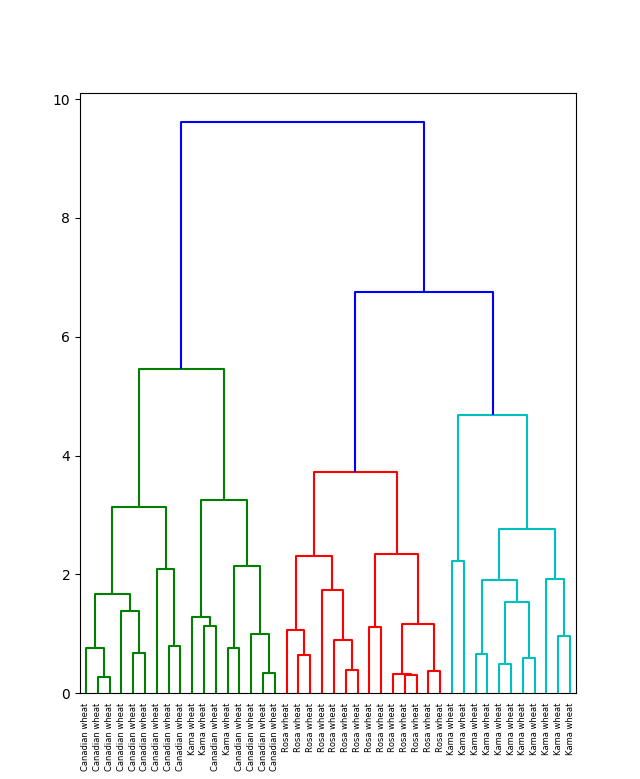
\includegraphics[width=7cm]{clasterization.png}
\end{itemize}

\end{document}
